\documentclass{homework}

\title{RAMLAB Internship \\ Progress Report}
\author{Ulf Torsten Kemmsies - 4794281  \\
MSc. Space Engineering - TU Delft}
\usepackage{geometry}
\usepackage{graphicx}
\graphicspath{ {./images/} }
\usepackage{amsmath}
\usepackage[table,xcdraw]{xcolor}
\usepackage{lscape}
\usepackage{multicol} % For multiple columns
\usepackage{capt-of} % For creating captions outside of floats

\begin{document}

\maketitle

\begin{abstract}

\end{abstract}

\begin{center}
Github repository: \url{test}    
\end{center}

\begin{multicols}{2} % Start two-column layout
\section{Introduction}

\begin{minipage}{\linewidth}
      \centering
      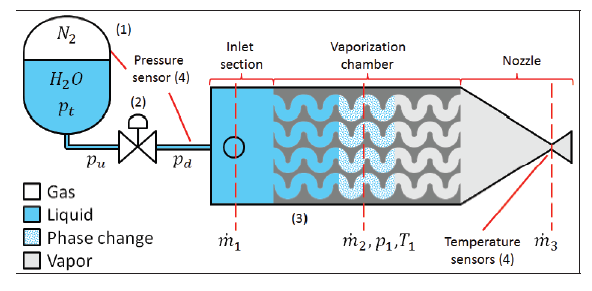
\includegraphics[width=\linewidth]{images/overview.png}
      \captionof{figure}{Picture example}
      \label{fig:model_overview}
  \end{minipage} 



% Figures \ref{fig:expansion_ratio_score} and \ref{fig:pressure_expansion_ratio} tell an interesting story about the relationship between the expansion ratio and other performance indicators: most of the top 1\% designs cluster around an expansion ratio of 4-7, while the pressure ratio in that range is around 0.025 and largely invariant to the expansion ratio.

% The equation for true thrust may hold the answer, since the negative pressure ratio is a contributing term. However, the divergence loss $\epsilon_{\text {div }}$ is greatly increased for large exit radii, and as the momentum loss is proportional to exit velocity $\Delta F_{\text {momentum }} \ \alpha \ u_e^2$, which is largely mediated by the exit Mach number, it may make sense that larger expansion radii have worse non-ideal thrust performance.

% \begin{minipage}{\linewidth}
%       \centering
%       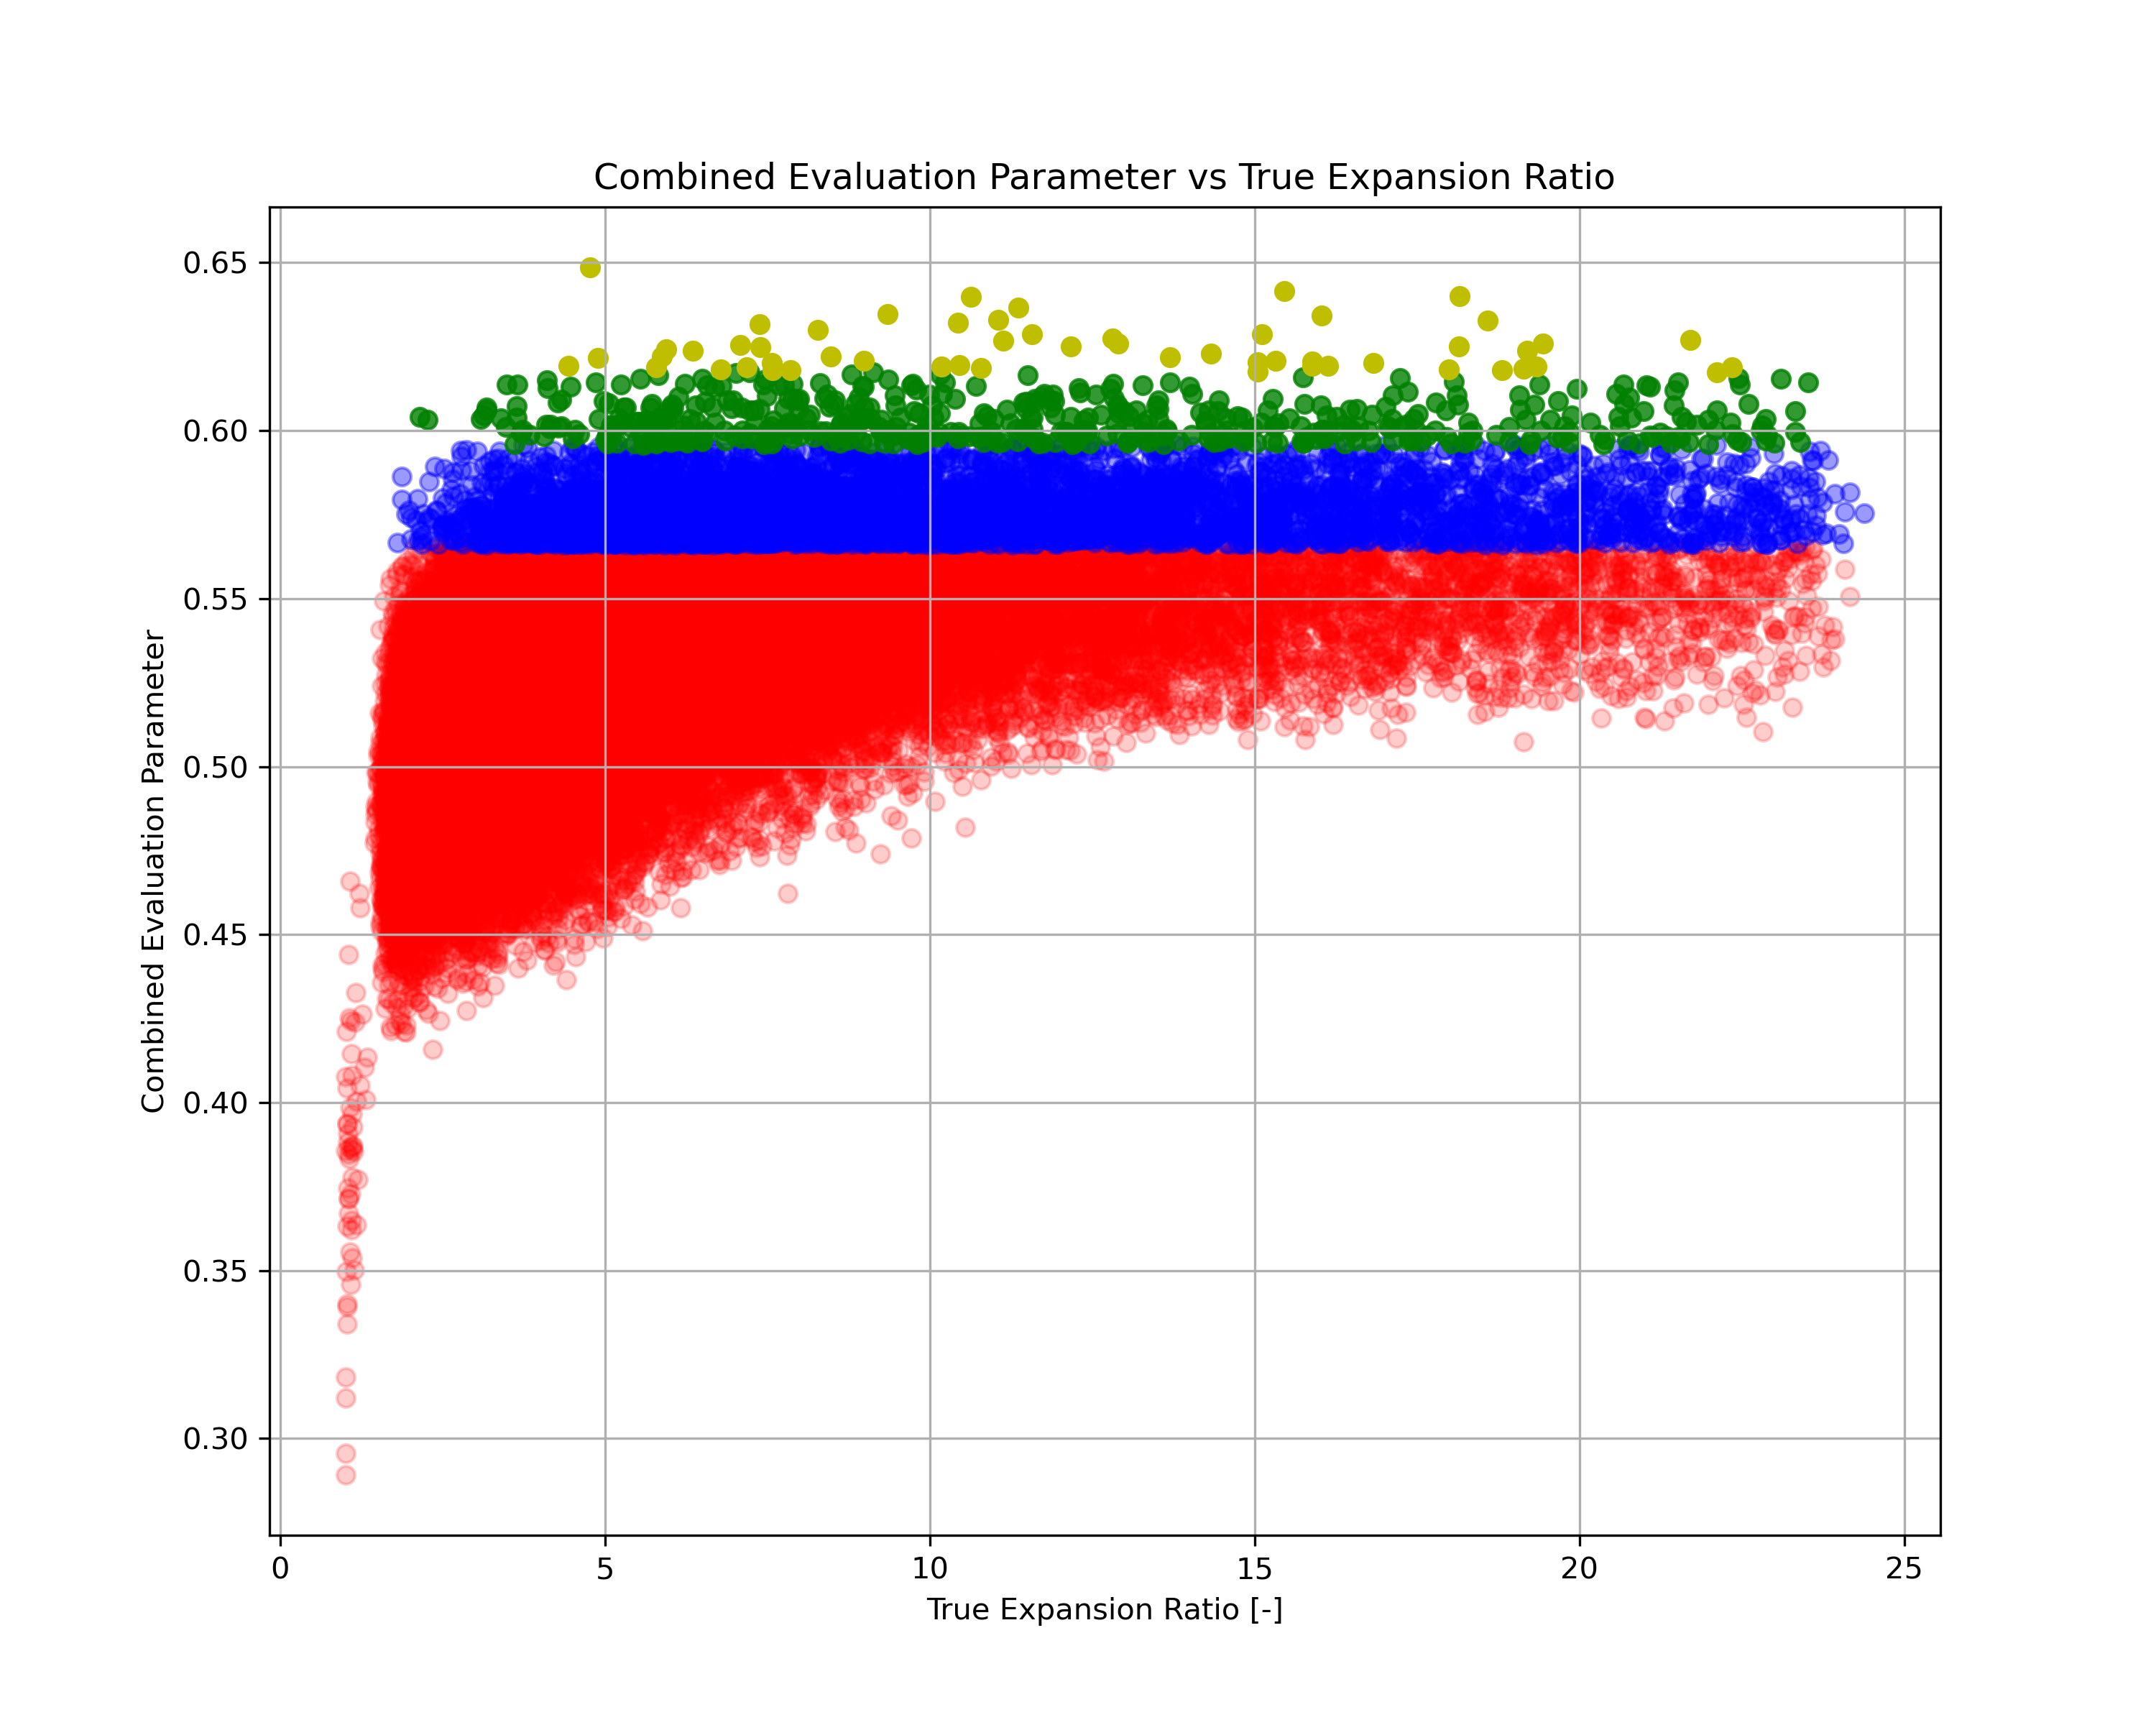
\includegraphics[width=\linewidth]{images/true_expansion_ratio_score.png}
%       \captionof{figure}{True Expansion Ratio vs. Evaluation Par.}
%       \label{fig:expansion_ratio_score}
%   \end{minipage}

%   \begin{minipage}{\linewidth}
%   \centering
%   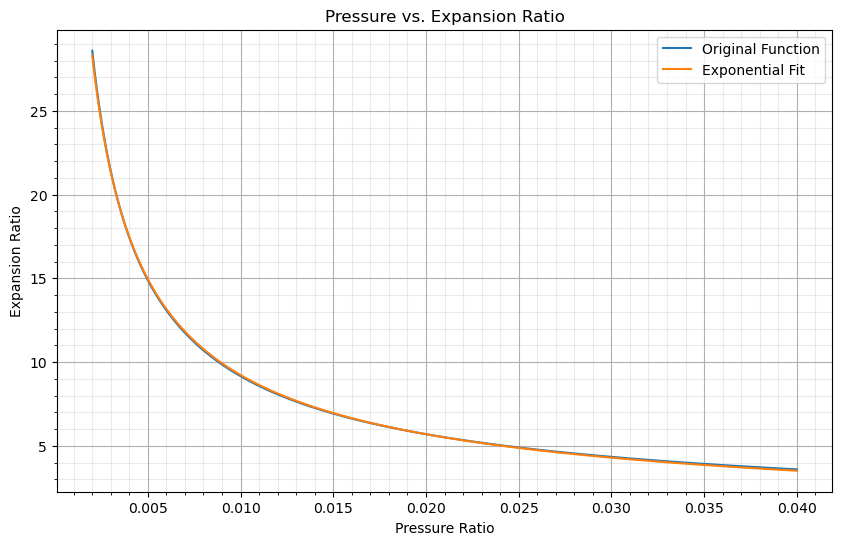
\includegraphics[width=\linewidth]{images/pressure_vs_expansion_ratio.png}
%   \captionof{figure}{Pressure Ratio vs. Expansion Ratio}
%   \label{fig:pressure_expansion_ratio}
% \end{minipage}


% \begin{align*}		    
% &F_{\text {true }}=\dot{m}_{true} \cdot \epsilon_{\text {div }} \cdot \\
% & \sqrt{2 \cdot \frac{\gamma}{\gamma-1} \cdot R_s \cdot \mathrm{T}_{\mathrm{c}} \cdot\left(1-\left(\frac{\mathrm{p}_{\mathrm{e}}}{\mathrm{p}_{\mathrm{c}}}\right)_{\text {true }}^{\frac{\gamma-1}{\gamma}}\right)}\\
% &-\Delta F_{\text {momentum }}
% \end{align*}

\bibliographystyle{plain} % We choose the "plain" reference style
\bibliography{refs} % Entries are in the refs.bib file

\end{multicols}
\end{document}
